% !TEX root = ./projekt.tex
%=========================================================================
% (c) Michal Bidlo, Bohuslav Křena, 2008

\chapter{Úvod}

\chapter{Definice a pojmy}

\section{Teorie množin}

\section{Teorie grafů}
\begin{defn}
  (Strom). \cite[str. 12]{Koutny}\\
  Strom je orientovaný acyklický graf, $G = (\Sigma, R)$, který má tyto
  tři vlastnosti: \\
  \indent
  $G$ má právě jeden uzel, do něhož nevstupují žádné hrany;
  tento uzel se nazývá kořen $G$ označovaný jako kořen($G$).\\
  \indent
  Jestliže $a \in \Sigma$ a $a \neq$ kořen($G$), potom $a$ je
  potomkem kořenu($G$) a vstupuje do něj právě jedna hrana.\\
  \indent
  Každý uzel $a \in \Sigma$ který není listem má svého přímého potomka,
  $b_1$ až $b_n$, řazené zleva doprava tak, že $b_1$ je
  nejlevějším přímým potomkem $a$ a $b_n$ je nejpravějším přímým
  potomkem $a$.
\end{defn}

\begin{defn}
  (Úroveň, cesta, řez, hranice, hloubka, elementární strom a podstrom). \cite[str. 12]{Koutny}\\
  Nechť $G = (\Sigma, R)$ je stromem.\\
  \indent
  Úroveň $l$, stromu $G$, je posloupnost $s$,
  všech uzlů se stejnou vzdáleností od kořene($G$).
  Jinými slovy, úroveň $l$, je posloupnost, $s = n_1 n_2 ... n_k$,
  taková, že existuje cesta v grafu o délce $\ell$ v $G$
  pro všechny posloupnost od kořene($G$)
  $ ... n_i$, pro $1 \leq i \leq k$ a $l \geq 1$.\\
  \indent
  Cesta $p$, stromu $G$, je posloupnost $s$, uzlů,
  kde první uzel je kořen($G$), poslední je listem a mezi každými
  dvěma následnými uzly v $s$ existuje hrana v $G$.
  Jinými slovy, cesta $p$ stromu $G$, je posloupnost,
  $s = n_1 n_2 ... n_k$, taková, že $s$ je cesta grafem
  o délce $k$ v $G$, kde $n_1 =$ kořen($G$) a $n_k$ je listem
  v $G$, pro $k \geq 1$.\\
  \indent
  Řez $c$, stromu $G$ je posloupnost $s$, uzlů takových,
  že každá cesta v $G$ má právě jeden uzel v $c$.
  Jinými slovy, řez $c$ je posloupnost, $s = n_1 n_2 ... n_k$,
  taková, že pro každou cestu $p = m_1 m_2 ... m_\ell$ stromu $G$,
  $|\{n_1, n_2, ..., n_k\} \cap \{m_1, m_2, ..., m_\ell\}| = 1$,
  pro $k, \ell \geq 1$.\\
  \indent
  Hranice stromu $G$, hranice($G$),
  je posloupnost listů $G$ řazených zleva do prava.\\
  \indent
  Hloubka stromu $G$, hloubka($G$), je délka nejdelší cesty v $G$;
  jestliže platí hloubka($G$)$ = 1$, potom je $G$ elementární strom.\\
  \indent
  Jestliže $G' = (\Sigma', R')$ představuje strom vyhovující těmto
  čtyřem podmínkám:
  $\Sigma' \neq \emptyset$;
  $\Sigma' \subseteq \Sigma$;
  $R' = (\Sigma' \times \Sigma')$;
  a jestliže v $G$ není žádný z uzlů v $\Sigma - \Sigma'$ potomkem
  uzlu v $\Sigma'$, potom je $G'$ podstromem $G$.
\end{defn}

\chapter{Formální jazyky}

Teorie formálních jazyků si bere za cíl formalizovat jazyky
(přirozené, programovací, matematické, ...) tak, abychom se mohli zabývat jejich
automatizovaným zpracováním.
Pojmy, které známe z lingvistiky jsou zde zobecněny a přesně definovány,
takže nemusí úplně odpovídat naší dosavadní představě.

\subsubsection*{Abeceda}

Základem jazyka je \term{abeceda}. V teorii formálních jazyků je obvykle značena
$\Sigma$ (sigma) a je definována jako konečná neprázdná množina, jejíž objekty
se nazývají \term{symboly}.

\subsubsection*{Řetězec}

Konečná posloupnost symbolů patřících do $\Sigma$ je \term{řetězec} nad $\Sigma$.
Zvláštním případem je $\varepsilon$ (epsilon), značící \term{prázdný řetězec} -
tedy takový, že neobsahuje žádný symbol.

\subsubsection*{Jazyk}

$\Sigma^*$ značí množinu všech řetězců, které je možné sestrojit nad abecedou $\Sigma$.
Jakákoliv podmnožina $L \subseteq \Sigma^*$ je \term{jazykem} nad abecedou $\Sigma$.
Jestliže \term{jazyk} představuje konečnou množinu řetězců, potom jej nazýváme \term{konečným jazykem},
v opačném případě \term{jazykem nekonečným}.

\subsubsection*{Gramatika}

Pokud se zabýváme nekonečnými jazyky, nemůžeme je vyjádřit jednoduchým výčtem jejich
řetězců. Místo toho definujeme \term{gramatiku}, která stanovuje pravidla pro generování
řetězců patřících do daného jazyka.\\

\noindent
\term{Gramatika} obecně obsahuje 4 části:
\begin{itemize}
  \item Množinu \term{neterminálních symbolů} $N$ (neterminálů), které slouží k označení syntaktických celků.
  \item Množinu \term{terminálních symbolů} $\Sigma$ (terminálů) - symboly, které jsou konečným výstupem. (abeceda)
  \item Množinu přepisovacích pravidel $P$.
  \item Počáteční (startovací) symbol $S \in N$.
\end{itemize}

\subsubsection*{Přepisovací pravidla}

\term{Přepisovací pravidlo} je složeno ze dvou řetězců $(\alpha, \beta)$,
složených z terminálů a neterminálů, přičemž $\alpha$ obsahuje alespoň jeden neterminál.
Zapisují se jako $\alpha \rightarrow \beta$.\\
Pravidla se aplikují od startovacího symbolu, kdy postupně přepisujeme řetězec tak že nahradíme
jakoukoliv část řetězce, která se nachází na levé straně některého pravidla za pravou stranu tohoto pravidla.
Tato operace se také nazývá \term{derivace}.
Řetězec upravujeme podle pravidel tak dlouho, až se v něm nacházejí pouze neterminály.

\begin{figure}[H]
  \label{img:rewriteRule}
  \centering
  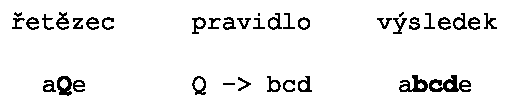
\includegraphics{fig/rewriteRule.pdf}
  \caption{Příklad derivace podle pravidla}
\end{figure}

\subsubsection*{Ekvivalence gramatik}
Dvě gramatiky označujeme jako \term{ekvivalentní}, pokud generují stejný jazyk.

\subsubsection*{Výpočetní model}

Výpočetní model lze definovat jako hypotetický přístroj,
který využíváme k řešení daného problému. Vlastnosti modelu určují,
jak sofistikované problémy je schopen řešit.

\subsubsection*{Hierarchie jazyků} \label{chomsky:hierarchy}

Omezením gramatiky lze zaručit to, že ji lze zpracovávat jednodušším
\term{Výpočetním modelem}. Jazyky se proto
dělí do tříd právě podle toho, jaký výpočetní model je dokáže zpracovat.\\

\noindent
Jedno z nejznámějších rozdělení je podle tzv. \term{Chomského hierarchie}:

\begin{itemize}
  \item \textbf{Gramatiky typu 0} (frázové/neomezené gramatiky)\\
  Zahrnují všechny formální gramatiky.\\
  Model pro zpracování se nazývá \term{Turingův stroj}.\\
  Tvoří třídu \term{rekurzivně spočetných jazyků}, zkratka \textbf{RE}.

  \item \textbf{Gramatiky typu 1} (kontextové gramatiky)\\
  Tyto gramatiky se skládají z pravidel typu $\alpha A\beta \rightarrow \alpha \gamma \beta$,
  kde $A$ je neterminál a $\alpha, \beta, \gamma$ jsou řetězce terminálů i neterminálů,
  přičemž $\gamma$ je neprázdný.\\
  Model pro zpracování se nazývá \term{lineárně ohraničený Turingův stroj}.\\
  Tvoří třídu \term{kontextových jazyků}, zkratka \textbf{CS}.

  \item \textbf{Gramatiky typu 2} (bezkontextové gramatiky)\\
  Skládají se z pravidel typu $A \rightarrow \gamma$, kde $A$ je neterminál a
  $\gamma$ řetězec terminálů a neterminálů.\\
  Model pro zpracování se nazývá \term{nedeterministický zásobníkový automat}.\\
  Tvoří třídu \term{bezkontextových jazyků}, zkratka \textbf{CF}.

  \item \textbf{Gramatiky typu 3} (regulární gramatiky)\\
  Skládají se z pravidel typu $A \rightarrow B$ a $A \rightarrow aB$,
  kde $A, B$ jsou neterminály a $a$ je terminál.\\
  Model pro zpracování se nazývá \term{konečný automat}.\\
  Tvoří třídu \term{regulárních jazyků}, zkratka \textbf{REG}.
\end{itemize}

\subsubsection*{Vyjadřovací síla jazyka}

Čím větší má jazyk vyjadřovací sílu, tím detailnější omezení je jeho
gramatika schopna klást na přijímané řetězce. Jsme tedy schopni jemněji rozlišovat,
které řetězce patří do jazyka a které ne.

V \term{Chomského hierarchii} jsou jazyky uspořádány tak, že slabší jazyk je
vždy podmnožinou silnějšího. Tedy například mezi Bezkontextové jazyky patří i
všechny Regulární jazyky.\\

\begin{figure}[H]
  \centering
  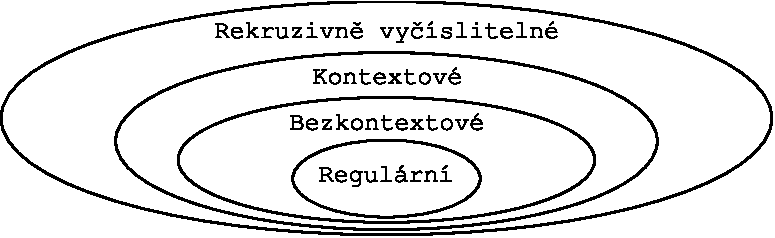
\includegraphics{fig/Chomsky.pdf}
  \caption{Schématické znázornění Chomského hieararchie}
\end{figure}


V této práci se budeme zabývat skupinami 2 a 3,
tedy bezkontextovými a regulárními jazyky. Tyto jazyky jsou prodrobněji
popsány v následujících kapitolách.

\section{Regulární jazyky}

Regulární jazyky jsou nejjednodušší formální jazyky v Chomského hierarchii.
I přesto si však našly široké využití v různých oblastech informačních technologií.
Využívají se např. pro pokročilé vyhledávání v textu nebo
pro rozdělení programovacího jazyka na základní jednotky.
V implementační části této práce jsou využity ke kontrole úrovní derivačního stromu,
také proto se jimi budeme hlouběji zabývat.

\begin{defn}
  (Regulární jazyk)\\
  Regulární jazyk nad abecedou $\Sigma$ lze definovat následovně:
  \begin{itemize}
    \item Prázdný jazyk $\emptyset$ je regulární.
    \item Pro každé $a$ z $\Sigma$ je $\{ a \}$ regulární.
    \item Jestliže $A$ a $B$ jsou regulární jazyky, poté všechny tyto jazyky jsou také regulární:
    $A \cup B$ (sjednocení), $AB$ (konkatenace) a $A^*$ (iterace).
  \end{itemize}
\end{defn}

\subsection{Konečné automaty}
Každý Regulární jazyk lze zpracovávat konečným automatem a každý konečný automat
lze vyjádřit regulárním jazykem.\\

Automat je pětice $M = (Q, \Sigma, R, s, F)$, kde:
\begin{itemize}
  \item $Q$ je množina stavů
  \item $\Sigma$ je \term{vstupní abeceda}
  \item $R$ je množina \term{přechodových pravidel}
  \item $s$ je \term{počáteční stav}
  \item $F$ je množina \term{konečných stavů}
\end{itemize}

Přechodová pravidla jsou ve tvaru $qa \rightarrow p$, kde $q, p$ jsou stavy a
$a$ je vstupní symbol. Pravidlo nám říká, že jsme-li ve stavu $q$ a na vstupu
máme symbol $a$, poté může automat přejít do stavu $p$.
Začínáme vždy v počátečním stavu a aby vstupní řetězec patřil do jazyka,
musíme skončit v jednom z konečných stavů.
Velkou výhodou je, že práce konečného automatu je paměťově velmi nenáročná, jelikož obsahuje pouze informaci o aktuálním
stavu.

\begin{exmp}
  Mějme konečný automat M1:
  \begin{lstlisting}[mathescape, escapeinside={(*}{*)}]
  M1 = (
    {s, q, f},        (* // množina stavů *)
    {a, b, c},        (* // abeceda *)
    {                 (* // množina pravidel *)
      sa $\rightarrow$ q1,
      qb $\rightarrow$ q,
      qc $\rightarrow$ f
    },
    s,                (* // počateční stav *)
    {f}               (* // množina ukončujících stavů *)
  )
  \end{lstlisting}
  A řetězec:
\begin{lstlisting}
  abbc
\end{lstlisting}

\noindent
Při kontrole vstupního řetězce budeme postupovat následovně:

\begin{enumerate}
  \item Nastavíme počáteční stav $s$
  \item Vstupním symbolem je 'a' - podle prvního pravidla přejdeme do stavu $q$
  \item Vstupním symbolem je 'b' - zůstáváme ve stavu $q$ (pr. 2)
  \item Vstupním symbolem je 'b' - zůstáváme ve stavu $q$ (pr. 2)
  \item Vstupním symbolem je 'c' - přejdeme do stavu $f$ (pr. 3)
  \item Jsme na konci řetězce - zkontrolujeme, zdali jsme v konečném stavu - řetězec byl automatem přijat,
  takže řetězec patří do jazyka generovaného automatem.
\end{enumerate}

\noindent
Během činnosti konečného automatu mohou nastat tyto chyby:

\begin{itemize}
  \item vstupní symbol nepatří do abecedy
  \item neexistuje pravidlo pro vstupní symbol a aktuální stav
  \item po přečtení posledního znaku se nenacházíme v konečném stavu
\end{itemize}
Ve všech těchto případech není vstupní řetězec přijat konečným automatem, tudíž nepatří
do jazyka generovaného automatem.\\

\noindent
Tento konečný automat lze také zobrazit pomocí následujícího grafu:

\begin{figure}[H]
  \centering
  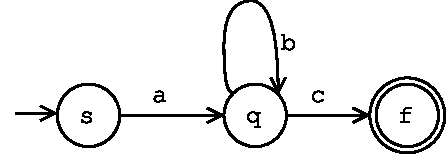
\includegraphics{fig/finiteAutomat.pdf}
\end{figure}

\end{exmp}

\noindent
Uveďme další příklad, který už nebude tak jednoduchý:
\begin{exmp}
  Mějme konečný automat M2:
  \begin{lstlisting}[mathescape, escapeinside={(*}{*)}]
  M2 = (
    {s, q1, q2, p1, p2, f1, f2},
    {a, b, c, d},
    {
      sa $\rightarrow$ q1,
      q1b $\rightarrow$ q2,
      q2c $\rightarrow$ f1,
      q1$\varepsilon$ $\rightarrow$ p1,
      p1b $\rightarrow$ p2,
      p2d $\rightarrow$ f2
    },
    s1,
    {f1}
  )
  \end{lstlisting}

  Za pozornost stojí hlavně čtvrté pravidlo s $\varepsilon$ přechodem.
  Toto pravidlo značí, že lze bez přijetí jakéhokoliv znaku přejít z jednoho stavu
  do druhého. Tyto pravidla se bohužel mohou v obecných gramatikách vyskytovat a
  způsobují potíže při zpracovávání automatu, jak bude vysvětleno dále.\\

  \noindent
  Pro větší názornost budeme nyní pracovat se schématem automatu:

  \begin{figure}[H]
    \centering
    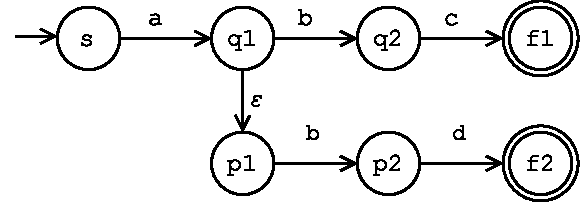
\includegraphics{fig/finiteAutomat1.pdf}
  \end{figure}

  Pokud se při zpracování ocitneme ve stavu $q1$ a vstupním symbolem bude 'b',
  není jasné, jestli máme použít 2. nebo 4. pravidlo. Museli bychom vyzkoušet jít oběma cestami
  a až zpětně bychom zjistili, která možnost byla správná. Tomuto jevu se v teorii
  formálních jazyků říká \term{nedeterminismus} a setkáme
  se s ním ještě několikrát.\\

  Nutno ale podotknout, že \term{nedeterminismus} neznamená to, že bychom nebyli schopni
  určit, jestli řetězec patří do daného jazyka. Ve skutečnosti totiž můžeme
  vyzkoušet všechna možná pravidla a zjistit, jestli z nich některé povede k úspěchu.
  Tato technika se také pro některé jazyky využívá a při zpracování
  přirozených jazyků se jí většinou nelze úplně vyhnout.
  Slepé zkoušení pravidel však vede k velkému zpomalení vyhodnocování,
  může totiž dojít k tomu, že se program bude větvit opakovaně
  a zpracování může dojít až k exponencionální složitosti.
  Např. programovací jazyky bývají navrženy tak, aby šly zpracovávat deterministicky,
  protože rychlost překladu je velmi důležitým faktorem pro jejich nasazení.\\


\end{exmp}

\subsection{Determinizace konečného automatu}

Z výše uvedených odstavců je zjevné, že je lepší se preventivně nedeterminismu
zbavit. Nejprve ukážeme demonstraci na tomto konkrétním příkladě a poté uvedeme
obecný algoritmus.\\

Abychom se zbavili $\varepsilon$ přechodů musíme vytvořit nový automat, který ale
generuje stejný jazyk (přijímá stejné řetězce)
jako ten původní. Takovéto dva automaty se označují jako \term{ekvivalentní}.
Protože můžeme z přechodu $q1$ kdykoliv přejít do $q2$ intuitivním řešením
je oba stavy spojit do jednoho. Pro zachování \term{ekvivalence}, musíme
do nového stavu přidat všechna pravidla, která vycházela z původních dvou stavů.
Nový automat bude vypadat takto:

\begin{figure}[H]
  \centering
  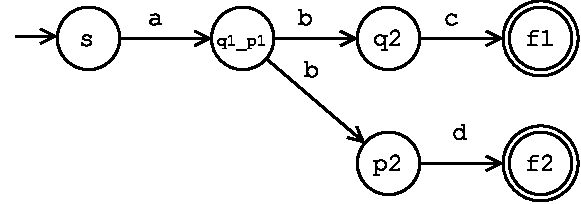
\includegraphics{fig/finiteAutomat1_1.pdf}
\end{figure}

Pokud si nové schéma dobře prohlédneme, odhalíme další zádrhel, který se nám
objevil v novém pravidle $q1\_p1$. Pokud je v tomto stavu na vstupu symbol 'b',
nevíme které pravidlo použít a máme tu opět \term{nedeterminismus}.
I tento problém lze naštěstí vyřešit obdobným způsobem:

\begin{figure}[H]
  \centering
  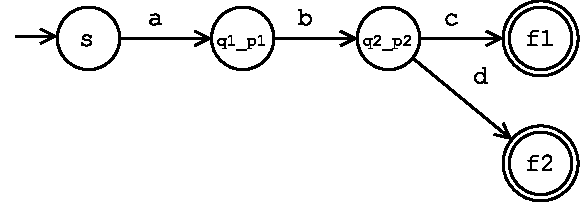
\includegraphics{fig/finiteAutomat1_2.pdf}
\end{figure}

\noindent
Tento automat můžeme označit jako \term{deterministický} a lze jej
s klidem implementovat.

\noindent
V tomto konkrétním případě jsme si pomohli intuicí, uveďme ale obecné algoritmy:\\

\begin{algorithm}[H]
  \caption{Stavy dostupné bez čtení ze stavů $E$ (\term{$\varepsilon$-uzávěr(E)})}
  \KwIn{Končný automat $M = (Q, \Sigma, R, s, F)$ a $E \subseteq Q$}
  \KwOut{\term{$\varepsilon$-uzávěr(E)}}

  \BlankLine
  \Begin{
    $\varepsilon$-uzávěr$(E)$ := $E$\;
    \Repeat{$\varepsilon$-uzávěr$(E)$ byl změněn}{
      $\varepsilon$-uzávěr$(E)$ := $\varepsilon$-uzávěr$(E)$ $\cup$ $\{p| q \rightarrow p
        \in R$ a $q \in \varepsilon$-uzávěr$(E)\}$
    }
  }
\end{algorithm}

\vspace{0.5cm}

\begin{algorithm}[H]
  \caption{Odstranění $\varepsilon$ pravidel}
  \KwIn{Končný automat $I = (Q_I, \Sigma_I, R_I, s_I, F_I)$ a $E \subseteq Q$}
  \KwOut{Konečný automat bez $\varepsilon$ pravidel $O$, ekvivalentní s $I$}

  \BlankLine
  \Begin{
    $Q_O$ := $Q_I$\;
    $\Sigma_O$ := $\Sigma_I$\;
    $s_O$ := $s_I$\;
    $F_O := \{q| q \in Q_I, \varepsilon$-uzávěr$(q) \cap F_I \neq \emptyset\}$\;
    $R_O := \{qa \rightarrow p | q \in Q_I, a \in \Sigma_I, oa \rightarrow p
      \in R_I$ pro všechna $o \in \varepsilon$-uzávěr$(q)$ v $I\}$
  }
\end{algorithm}

\vspace{0.5cm}

\begin{algorithm}[H]
  \caption{Odstranění nedeterminismu}
  \KwIn{Končný automat bez $\varepsilon$-přechodů $M = (Q, \Sigma, R, s, F)$}
  \KwOut{Deterministický KA: $D = (Q_D, \Sigma, R_D, s_D, F_D)$ ekvivalentní s $M$}

  \BlankLine
  \Begin{
    $s_D := \{s\}$\;
    $Q_{new} := \{s_D\}$\;
    $R_D := \emptyset$\;
    $Q_D := \emptyset$\;
    $F_D := \emptyset$\;
    \Repeat{$Q_{new} = \emptyset$} {
      nechť $Q' \in Q_{new}$\;
      $Q_{new} := Q_{new} - \{Q'\}$\;
      $Q_D := Q_D \cup {Q'}$\;
      \ForAll{$a \in \Sigma$}{
        $Q'' := \{q | p \in Q', pa \rightarrow q \in R\}$\;
        \If{$Q'' \neq \emptyset$}{
          $R_D := R_D \cup \{ Q' a \rightarrow Q'' \}$\;
        }
        \If{$Q'' \notin Q_D \cup \{\emptyset\}$}{
          $Q_{new} := Q_{new} \cup \{Q''\}$\;
        }
      }
      \If{$Q' \cap F \neq \emptyset$}{
        $F_D := F_D \cup \{ Q'\}$
      }
    }
  }
\end{algorithm}

\vspace{0.5cm}

Tyto algoritmy jsou definovány pro jakýkoliv Konečný automat, tedy jakýkoliv KA
lze převést na Deterministický KA \cite[str. 39]{MedunaIFJ}.
Z toho vyplývá, že jakýkoliv Regulární jazyk lze zpracovávat deterministicky,
což u jazyků z ostatních tříd \term{Chomského hierarchie} neplatí.\\

Existují také další transformace Konečného automatu, jako např.
odstranění nedostupných stavů nebo minimalizace. V této práci však
nebudou využívány a proto zde nejsou více rozebírány.\\

\subsection*{Na co konečné automaty nestačí}

\begin{exmp}
  \label{exmp:brackets}

  Řekněme, že chceme konečným automatem kontrolovat,
  jestli matematický výraz obsahuje stejné množství
  otevíracích závorek jako uzavíracích a jestli jsou ve správném pořadí.\\
  Příklady řetězců:
  \begin{itemize}
    \item '(())' - v pořádku
    \item '(()())' - v pořádku
    \item '(()' - špatně
    \item ')(' - špatně
  \end{itemize}

  Příklad si zjednodušíme tak, že nebudeme uvažovat žádná čísla ani znaky uvnitř
  závorek.\\

  Když tedy přečteme první '(' musíme přejít do stavu, který značí
  "čekám jednu uzavírací závorku" (pro větší přehlednost budeme tento stav označovat $[)]$)
  a když je dalším znakem ')' přejít do konečného stavu.
  Tento konečný automat lze znázornit takto:

  \begin{figure}[H]
    \centering
    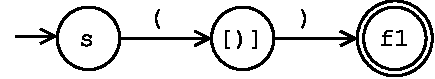
\includegraphics{fig/finiteAutomat2.pdf}
  \end{figure}

  Tento automat bude fungovat bez problému pro řetězec '()',
  my ale chceme zpracovávat i zanořené závorky a na to tento automat zatím nestačí.
  Pokud tedy chceme univerzálnější automat, stačí přidat další stav:

  \begin{figure}[H]
    \centering
    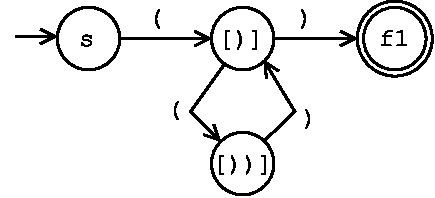
\includegraphics{fig/finiteAutomat2_1.pdf}
  \end{figure}

  Zde již zvládneme i závorky s jedním zanořením. Problémem ovšem je, že
  pro každé nové zanoření musíme přidat nový stav.
  Kdybychom tedy chtěli zpracovávat jakýkoliv počet zanoření (tedy potenciálně $\infty$),
  musel by automat obsahovat nekonečné množství stavů.
  Vidíme, že problémem Konečného automatu je, že může obsahovat pouze konečný
  počet stavů (a každý musíme ručně definovat).
  Zde tedy vidíme příklad jazyka, který nejde zpracovávat Konečným automatem
  a z toho vyplívá, že není ani Regulárním jazykem.
  Řekněme si rovnou, že bezkontextové jazyky tento problém řeší a k tomuto
  příkladu se ještě vrátíme.

\end{exmp}

\section{Bezkontextové jazyky}

Bezkontextový jazyk je definován Bezkontextovou gramatikou.
Jak jsme již uvedli v \term{Chomského hierarchii} (str. \pageref{chomsky:hierarchy}),
tyto gramatiky obsahují pravidla ve tvaru $A \rightarrow \gamma$, kde $A$ je neterminál a
$\gamma$ řetězec terminálů a neterminálů.

\subsection{Bezkontextové gramatiky}

Pokračujme nyní v příkladu \ref{exmp:brackets} a ukažme si, jak ho lze
vyjádřit pomocí bezkontextové gramatiky a zpracovávat zásobníkovým automatem.\\

Chceme tedy vyjádřit výraz tvořený závorkami, pomocí gramatických pravidel.
Označme dvojici závorek jako výraz = neterminál $E$. Gramtické pravidlo tedy bude
vypadat takto:
\[E \rightarrow ()\]
Nyní bychom ale chtěli vyjádřit, že uvnitř závorek může být další výraz, to
lze udělat tímto rekurzivním způsobem:
\[E \rightarrow (E)\]
Zkusme nyní rozgenerovávat výraz E, tak jak to bylo naznačeno na Obr. \ref{img:rewriteRule},
tedy pomocí přepisování neterminálů:
\begin{lstlisting}
  1.        E
  2.       (E)
  3.      ((E))
  4.     (((E)))
  5.       ...
\end{lstlisting}
Vidíme, že zanořování, které nám dělalo problémy u regulárních jazyků, zde vyjádříme bez problému,
ještě by to však chtělo několik vylepšení.
Můžeme si všimnout, že rozgenerovávání by se vlastně mělo provádět do nekonečna,
protože neterminálu E se nyní nelze zbavit. To lze vyřešit přidáním tzv.
$\varepsilon$-pravidla:
\[E \rightarrow \varepsilon\]
To nám říká, že neterminál E je možno kdykoliv vymazat. Dále bychom ještě chtěli,
aby se za závorkou mohla vyskytovat další závorka, např. '(()())'.
Stačí přidat do výrazu další rekurzi:
\[E \rightarrow (E)E\]
Všimněme si ještě, že začínáme od symbolu $E$, který lze vymazat pomocí
$\varepsilon$-pravidla, přijímáme tedy i prázdný řetězec. Pokud bychom chtěli
vyjádřit, že celý výraz musí být alespoň v jedněch závrokách lze to udělat
přidáním speciálního počátečního pravidla:
\[S \rightarrow (E)\]
Nyní tedy budeme začínat od symbolu S. Označme si tuto gramatiku jako
$G$ a vyjádřeme ji formálně:
\begin{lstlisting}[mathescape, escapeinside={(*}{*)}]
  G = (
    {S, E},           (* // množina neterminálů *)
    {(, )},           (* // množina terminálů *)
    {                 (* // množina pravidel *)
      S $\rightarrow$ (E),
      E $\rightarrow$ (E)E,
      E $\rightarrow$ $\varepsilon$
    },
    S                 (* // počáteční symbol *)
  )
\end{lstlisting}

Je zřejmé, že bezkontextovými jazyky jsme schopni popsat mnohem
složitější jazyky, než regulárními jazyky. Daní za větší \term{vyjadřovací sílu}
je ale znatelně složitější zpracování těchto jazyků.

\subsection{Zásobníkové automaty}

Zásobníkový automat rozšiřuje \term{Konečný automat} o zásobník, kam lze
ukládat symboly (terminály i neterminály). Pro rozhodnutí, jaké pravidlo použít,
využívá vedle vstupního symbolu i symbol na vrcholu zásobníku. V rámci vykonání
přechodu lze zároveň manipulovat se zásobníkem.\\


\subsection{Derivační strom}
Při aplikaci gramatiky na řetězec jde vlastně o ověření,
jestli lze z počátečního symbolu,
postupnou derivací (aplikací pravidel gramatiky) získat daný řetězec.
Mějme například gramatiku:

\begin{lstlisting}[mathescape]
  G = (
    {S, a, b, c},
    {a, b, c},
    {
      S $\rightarrow$ aSc,
      S $\rightarrow$ b
    },
    S
  )
\end{lstlisting}
\noindent
Pravidla této gramatiky lze vyjádřit pomocí elementárního stromu,
kde levá strana je kořen a pravá strana představuje jeho potomky.
Např. první pravidlo z gramatiky $G$ lze znázornit stromem takto:
\begin{figure}[H]
  \centering
  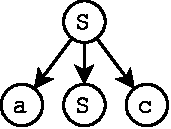
\includegraphics{fig/RuleTree1.pdf}
\end{figure}

\noindent
Pro menší velikost grafu budeme ale pravidla zjednodušeně znázorňovat takto:

\begin{figure}[H]
  \centering
  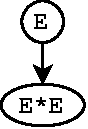
\includegraphics{fig/RuleTree2.pdf}
\end{figure}

\noindent
Pro příklad postupné derivace mějme řetězec $s$:

\begin{lstlisting}
  aaabccc
\end{lstlisting}

\noindent
Nyní zkusíme postupně aplikovat pravidla na počáteční symbol,
tak abychom získali řetězec $s$
(v komentáři jsou uvedena pravidla, která byla použita):

\begin{lstlisting}[mathescape]
     S
    aSc                   //S $\rightarrow$ aSc
   aaScc                  //S $\rightarrow$ aSc
  aaaSccc                 //S $\rightarrow$ aSc
  aaabccc                 //S $\rightarrow$ b
\end{lstlisting}

\noindent
Touto posloupností derivací jsme byli schopni dosáhnout kontrolovaného řetězce $s$,
daný řetězec tedy patří do gramatiky. Výše zobrazené derivace lze zobrazit
i jinak a to pomocí tzv. \term{Derivačního stromu}:

\begin{figure}[H]
  \centering
  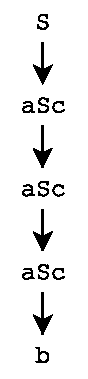
\includegraphics{fig/Derivations1.pdf}
\end{figure}

\noindent
Pro větší názornost ukažme ještě stejný strom s přiřazenými symboly k původnímu
řetězci a vyznačenými jednotlivými úrovněmi.

\begin{figure}[H]
  \centering
  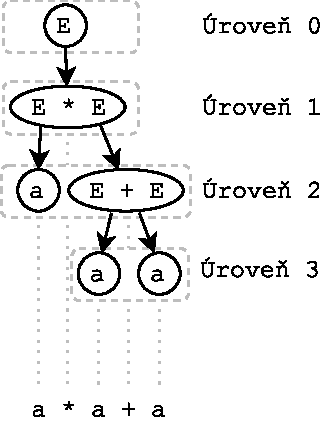
\includegraphics{fig/Derivations2.pdf}
\end{figure}

\begin{defn}
  (Derivační strom). \cite[str. 92]{MedunaIFJ}\\
  Nechť $G = (\Sigma, R)$ je Bezkontextová gramatika.\\
  \begin{enumerate}
    \item Pro $l$: $A \rightarrow x \in R, A\langle x\rangle$ je strom pravidla, které reprezentuje $l$.
    \item Derivační strom reprezentující derivace v $G$ je definován rekurzivně:
    \begin{enumerate}
      \item Strom s jedním uzlem $X$ je derivační strom odpovídající $X \Rightarrow^0 X$ v $G$, kde $X \in \Sigma$.
      \item Nechť $d$ je derivační strom reprezentující
            $A \Rightarrow^0 uBv$ [$\rho$] s hranicí($d$) $ = uBv$, a nechť $l: B \rightarrow z \in R$.
            Derivační strom, který reprezentuje
            \begin{align}
                A & \Rightarrow^* uBv [\rho] \nonumber\\
                  & \Rightarrow \hphantom{*} uzv [l] \nonumber
            \end{align}
            je získán nahrazením ($|u|+1$)-tého listu v $d$, $B$, stromem pravidla odpovídajícho $l$, $B\langle z\rangle$
    \end{enumerate}
    \item Derivační strom v $G$ je jakékoliv $t$, pro které existuje derivace odpovídající $t$ (viz 2.).
  \end{enumerate}
\end{defn}

\chapter{Zpracování jazyků řízených stromy}

\section{Omezení úrovní derivačního stromu}

V této části práce je vysvětleno, jak lze omezit derivační stromy a tím zvýšit
sílu dané gramatiky.
Teoretická část této sekce vychází převážně z práce Ing. Koutného\cite{Koutny}.\\

\subsection{Definice}

\begin{defn}
  (Gramatiky řízené stromy) \cite[str. 28]{Koutny}\\
  Gramatika řízená stromem je dvojice $(G, R)$, kde $G = (V, T, P, S)$
  je řízená gramatika a $R \subseteq V^*$ kontrolní jazyk.
\end{defn}

\begin{defn}
  (Jazyky řízené stromy) \cite[str. 28]{Koutny} \label{jazykyRS}\\
  Nechť $(G, R)$ je gramatika řízená stromem.
  Jazyk generovaný $(G, R)$ je značen jako $L(G, R)$ a definován jako:
  \begin{adjustwidth}{0.5cm}{0.5cm}
    $L(G, R) = \{x: x \in L(G, R)$ a existuje derivační strom $t$ pro
    každé $x$ v $G$ takový, že každé slovo získané konkatenací
    všech symbolů na kterékoliv úrovni $t$ (kromě poslení) zleva doprava,
    patří do $R \}$.\\
  \end{adjustwidth}
\end{defn}

\noindent
V této práci se zabýváme především gramatikami bezkontextovými, protože
je lze relativně snadno zpracovávat a kontrolní jazyk bude regulární.
Jinými slovy, zabýváme se gramatikami $(G, R)$, kde G je bezkontextová gramatika
a R je regulární jazyk.

\subsection{Příklady}

Pro lepší porozumění následuje podrobný praktický příklad, jak lze
ověřovat příslušnost řetězce do dané gramatiky řízené stromem.

\begin{exmp}
  Mějme stromem řízený jazyk $L(G, R)$, kde:
  \begin{lstlisting}
  G = (
    {S, A, B, C, a, b, c},
    {a, b, c},
    {
      S -> ABC,
      A -> aA,
      A -> a,
      B -> bB,
      B -> b,
      C -> cC,
      C -> c
    },
    S
  ),
  R = {S, ABC, aAbBcC}
  \end{lstlisting}
  \noindent
  A řetězec:

  \begin{lstlisting}
  aabbcc
  \end{lstlisting}

  \noindent
  Nejprve sestavíme derivační strom pro daný řetězec, poté projdeme všechny
  jeho úrovně (kromě poslední, viz. Definice \ref{jazykyRS}) a
  ověříme, že patří do kontrolního jazyka $R$.

  \begin{figure}[H]
    \centering
    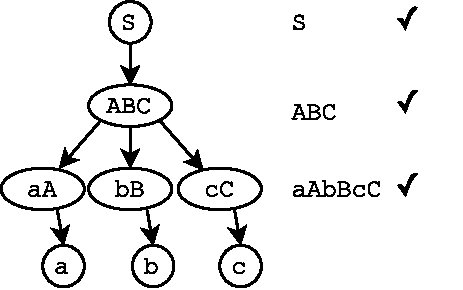
\includegraphics{fig/TreeControlledGrammar1.pdf}
  \end{figure}

  \noindent
  Z grafu je zřejmé, že v tomto případě řetězec patří do jazyka $L$.
  Zkusme však ještě jiný případ pro tento řetězec:

  \begin{lstlisting}
  aabcc
  \end{lstlisting}

  \noindent
  A jemu odpovídající derivační strom:
  \begin{figure}[H]
    \centering
    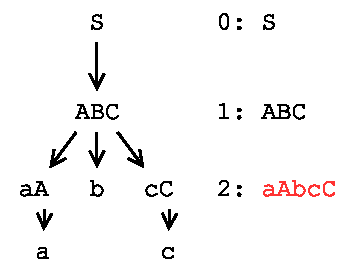
\includegraphics{fig/TreeControlledGrammar2.pdf}
  \end{figure}

  \noindent
  V tomto případě úroveň 2 derivačního stromu nepatří do kontrolního jazyka $R$,
  proto tento řetězec nepatří do jazyka $L$.
\end{exmp}

\section{Syntaktická analýza}
V předchozích kapitolách jsme se vždy zabývali pouze tím, jak pracovat s derivačním stromem,
ale ne jakým způsobem ho sestavit pro daný řetězec a gramatiku.
Metody řešící tento problém jsou již podrobně prozkoumané a obecně známé,
proto není tolik vysvětlován jejich princip, ale spíše jejich vlastnosti, mající
vliv na podobu derivačního stromu.\\

Při návrhu syntaktického analyzátoru se vždy objeví otázka, zdali je lepší
při konstrukci derivačního stromu postupovat od kořene (shora dolů) nebo od
zkoumaného řetězce (zdola nahoru). Odpověď na tuto otázku není jednoznačná,
což je vidět i na široce používaných analyzátorech programovacích jazyků,
kdy se tato technika liší projekt od projektu.\\

V případě tohoto projektu je tomu nejinak, a proto v této části budeme rozebírat
obě alternativy, aby byly zřejmé jejich výhody i nevýhody.

\subsection{Shora dolů}

\subsection{Zdola nahoru}
\chapter{Implementace}

%=========================================================================
